\documentclass{beamer}

% Theme choice:
\usetheme{CambridgeUS}
\usepackage{amsmath}
\usepackage{graphicx}
\usepackage{array}
\newcolumntype{P}[1]{>{\centering\arraybackslash}p{#1}}

% Title page details: 
\title{AI1110: Probability and Random Variables}
\subtitle{Random Numbers}
\author{Rishit D (cs21btech11053)}
\institute{IIT Hyderabad}
\date{\today}


\begin{document}

% Title page frame
\begin{frame}
	\titlepage 
\end{frame}

%Outline
\begin{frame}{Outline}
	\tableofcontents
\end{frame}

%Sections
\section{Problem 1}

\subsection{Problem 1.2}

\begin{frame}
	\frametitle{1.2: CDF of U - Python Plot}
	\begin{figure}
		\centerline{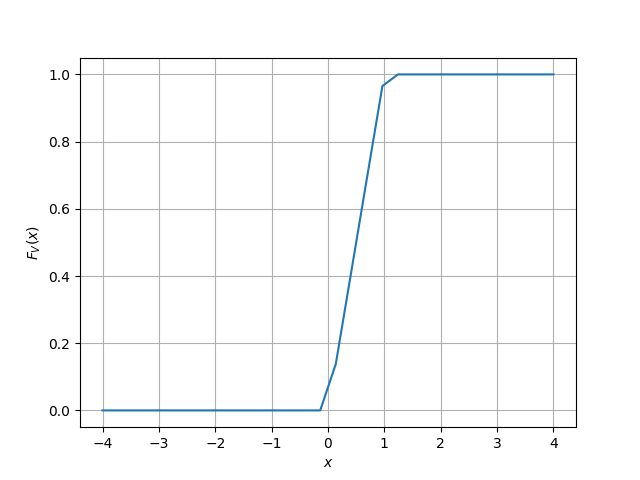
\includegraphics[width=\textheight]{../figs/uni_cdf.png}}
		\label{fig1}
	\end{figure}
	
\end{frame}	
\subsection{Problem 1.3}

%PDF
\begin{frame}
	\frametitle{1.3: Probability Density of U}

	Given $U$ is a uniformly distributed random variable over the interval $(0, 1)$, we have the density function $p_U(x)$:

	\begin{align}
		p_U(x) = 
		\begin{cases}
			1, & x \in (0, 1) \\
			0, & otherwise
		\end{cases}
		\label{eq:PDF}
	\end{align}
\end{frame}

%Getting Distribution
\begin{frame}
	\frametitle{1.3: Getting $F_U(x)$}

	We know

	\begin{align}
		F_U(x) = \int_{-\infty}^{x} p_U(x) \,dx
		\label{eq:Relation}
	\end{align}

\end{frame}

%CDF
\begin{frame}
	\frametitle{1.3: Theoretical Expression for Distribution of U}
	Given $U$ is a uniformly distributed random variable over the interval $(0, 1)$, we have the following expression for $F_U(x)$:
	
	\begin{align}
		F_U(x) = 
		\begin{cases}
			0, & x \in (-\infty, 0) \\
      			x, & x \in (0, 1) \\
      			1, & x \in (1, \infty)
    		\end{cases}
	\end{align}
\end{frame}

\subsection{Problem 1.5}
%PDF
\begin{frame}
	\frametitle{1.5: Definitions}

	We are given that

	\begin{align}
		E[U^k] = \int^{\infty}_{-\infty} x^k dF_U(x)
	\end{align}

	This can be alternatively wriiten as
	\begin{align}
		E[U^k] = \int^{\infty}_{-\infty} x^k p_U(x) \,dx
		\label{eq: Expected}
	\end{align}

\end{frame}

%Mean
\begin{frame}
	\frametitle{1.5: Finding Mean}
	We know that mean $\mu$ is given by $E(U)$. Hence

	\begin{align}
		\mu = \int_{-\infty}^{\infty} x p_U(x) \,dx
		\label{eq:Relation_1}
	\end{align}

	\begin{align}
		\mu &= \int_{0}^{1} x \,dx \\
		&= \frac{x^2}{2} \big|^{1}_{0} \\
		&= \frac{1}{2} 
		\label{eq: Mean}
	\end{align}

\end{frame}

%Variance
\begin{frame}
	\frametitle{1.5: Finding Variance}
	We know

	\begin{align}
		var(U) = E((U - E(U))^2)
	\end{align}

	This can also be represented as
	\begin{align}
		var(U) &= E(U^2 - 2E(U)U + (E(U))^2) \\
		&= E(U^2) - 2(E(U))^2 + (E(U))^2 \\
		&= E(U^2) - (E(U))^2
		\label{eq: Relation_2}
	\end{align}
	
\end{frame}

%Variance
\begin{frame}
	\frametitle{1.5: Finding Variance}
	We can evaluate $E(U^2)$ using \eqref{eq: Expected} as:
	
	\begin{align}
		E(U^2) &= \int_{-\infty}^{\infty} x^2 p_U(x) \,dx \\
		&= \int_{0}^{1} x^2 \,dx \\
		&= \frac{x^3}{3} \big|^{1}_{0} \\
		&= \frac{1}{3}
	\end{align}

	Using \eqref{eq: Mean} and \eqref{eq: Relation_2} we have
	\begin{align}
		var(U) = \frac{1}{3} - \frac{1}{4} = \frac{1}{12}
	\end{align}

\end{frame}


\section{Problem 2}

\subsection{Problem 2.2}

\begin{frame}
	\frametitle{2.2: CDF of X - Python Plot}
	\begin{figure}
		\centerline{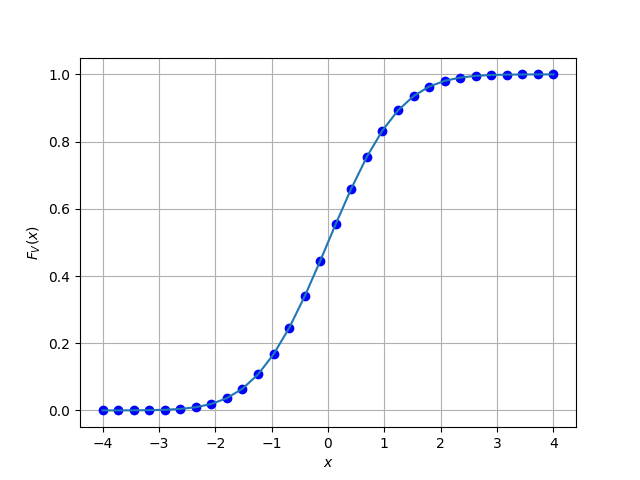
\includegraphics[width=\textheight]{../figs/gau_cdf.png}}
		\label{fig2}
	\end{figure}
	
\end{frame}	

\subsection{Problem 2.3}

\begin{frame}
	\frametitle{2.3: PDF of X - Python Plot}
	\begin{figure}
		\centerline{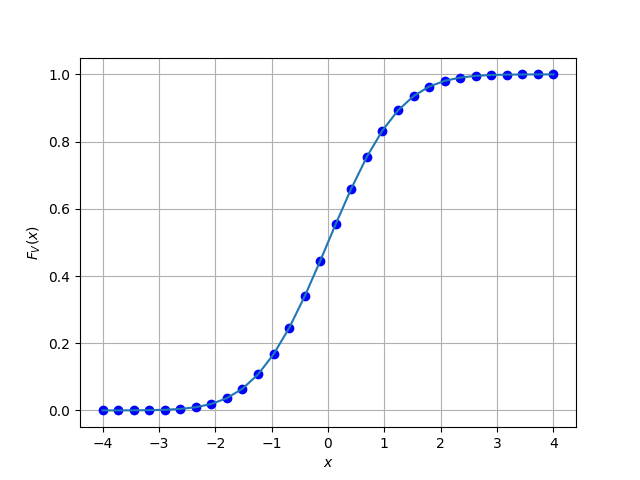
\includegraphics[width=\textheight]{../figs/gau_cdf.png}}
		\label{fig3}
	\end{figure}
	
\end{frame}

\subsection{Problem 2.5}

%Problem: PDF
\begin{frame}
	\frametitle{2.5: Probability Density}
	For random variable $X$, we have been given the density function as follows
	\begin{align}
		p_X(x) = \frac{1}{\sqrt{2\pi}}\exp{\frac{-x^2}{2}} 
		\label{eq:PDF_2}
	\end{align}
\end{frame}

%Getting Distribution: CDF
\begin{frame}
	\frametitle{2.5: Getting $F_X(x)$}

	Given
	\begin{align}
		F_X(x) = \int_{-\infty}^{x} p_X(x) \,dx
		\label{eq:Relation_3}
	\end{align}

	We have, using 
	\eqref{eq:Relation_3} and 
	\eqref{eq:PDF_2}
	\begin{align}
		F_X(x) = \int_{-\infty}^{x} \frac{1}{\sqrt{2\pi}}\exp{\frac{-x^2}{2}} \,dx
	\end{align}

\end{frame}

%Mean
\begin{frame}
	\frametitle{2.5: Mean}
	Mean for random variable $X$ is given by:
	
	\begin{align}
		\mu_x &= E(X) \\
		&= \int^{\infty}_{-\infty} x p_X(x) \,dx \\
		&= \int^{\infty}_{-\infty} x \frac{1}{\sqrt{2\pi}}\exp{\frac{-x^2}{2}} \,dx \\
		&= 0
	\end{align}

	Note that the integral
	\begin{align}
		\int^a_{-a} f(x) \,dx
	\end{align}
	becomes 0, when $f(x)$ is odd.

\end{frame}

%Variance
\begin{frame}
	\frametitle{2.5: Variance}
	Variance for random variable $X$ is given by:

	\begin{align}
		var(X) = E(X^2) - (E(X))^2
		\label{eq: MeanVar}
	\end{align}

	We evaluate $E(X^2)$ as follows:

	\begin{align}
		E(X^2) &= \int^{\infty}_{-\infty} x^2 p_X(x) \,dx \\
		&= x \int x p_X(x) \,dx \Big|^{\infty}_{-\infty} - \int \frac{dx}{dx} (\int x p_X(x) \,dx) \,dx\Big|^{\infty}_{-\infty} \\
		&= x \times -\sqrt{\frac{2}{\pi}} \exp{\frac{-x^2}{2}}\Big|_{-\infty}^{\infty} - \int^{\infty}_{-\infty} -\sqrt{\frac{2}{\pi}} \exp{\frac{-x^2}{2}} \,dx \\
		&= 1
		\label{eq: MeanSec}
	\end{align}

\end{frame}

\begin{frame}
	\frametitle{2.5: Variance}
	Hence using \eqref{eq: MeanVar} and \eqref{eq: MeanSec}, we have

	\begin{align}
		var(X) &= E(X^2) - (E(X))^2 \\
		&= 1 - 0^2
		&= 1
	\end{align}
\end{frame}

	
\section{Problem 3}

\subsection{Problem 3.1}

\begin{frame}
	\frametitle{3.1: CDF of V - Python Plot}
	\begin{figure}
		\centerline{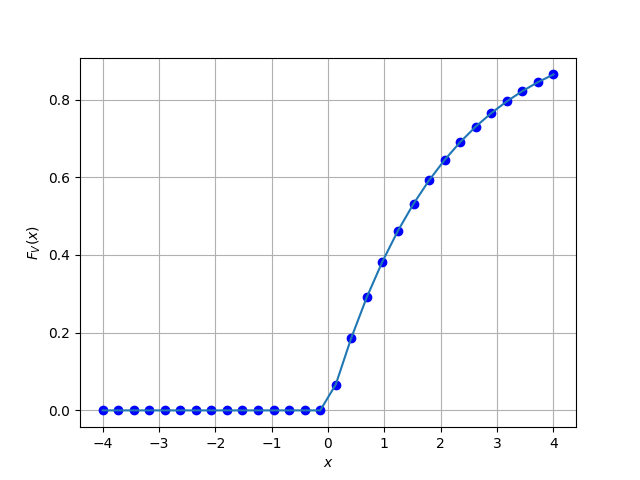
\includegraphics[width=\textheight]{../figs/log_cdf.png}}
		\label{fig4}
	\end{figure}
	
\end{frame}	

\subsection{Problem 3.2}

%PDF
\begin{frame}
	\frametitle{3.2: Relation between U and V}

	We have been given that random variable $V$ is a function of the random variable $U$ as follows:
	
	\begin{align}
		V = -2\ln{(1 - U)}
		\label{eq:FuncRV}
	\end{align}

	Note that the obtained distribution function (CDF) for random variable $U$ is:

	\begin{align}
		F_U(x) = 
		\begin{cases}
			0, & x \in (-\infty, 0) \\
			x, & x \in (0, 1) \\
			1, & x \in (1, \infty)
		\end{cases}
		\label{eq:CDF_U}
	\end{align}
\end{frame}

%Getting Distribution for V
\begin{frame}
	\frametitle{3.2: Getting $F_V(x)$}

	We know for any random variable $X$

	\begin{align}
		F_X(x) = \Pr(X \leq x)
		\label{eq:CDF_Def}
	\end{align}

	Hence, we can write using \eqref{eq:FuncRV} and \eqref{eq:CDF_Def}

	\begin{align}
		F_V(x) &= \Pr(V \leq x) \\
		&= \Pr(-2\ln{(1 - U)} \leq x)\\
		&= \Pr(\ln{(1 - U)} \geq \frac{-x}{2})\\
		&= \Pr(1 - U \geq \exp{\frac{-x}{2}})\\
		&= \Pr(U \leq 1 - \exp{\frac{-x}{2}})\\
		&= F_U(1 - \exp{\frac{-x}{2}})
		\label{eq: CDF_Rel}
	\end{align}

\end{frame}

%CDF
\begin{frame}
	\frametitle{3.2: Final expression for $F_V(x)$}
	Note that the function $f(x) = 1 - \exp{\frac{-x}{2}}$ follows:
	\begin{align}
		f(x) \in
		\begin{cases}
			{0}, & x \in (-\infty, 0) \\
			(0, 1) & x \in (0, \infty)
		\end{cases}
	\end{align}

	Hence we can write
	\begin{align}
		F_V(x) = 
		\begin{cases}
			0, & x \in (-\infty, 0) \\
			1 - \exp{\frac{-x}{2}}, & x \in (0, \infty)
    		\end{cases}
	\end{align}
\end{frame}

\end{document}

